\documentclass[11pt,twocolumn]{article}
\usepackage[margin=0.78in]{geometry}
\usepackage{graphicx}
\usepackage{amsmath}
\usepackage{times}
\usepackage{url}
\emergencystretch=2em

\pdfinfo{
  /Title (When Prompt Interfaces Fail: A Gated Study of Reference-Guided Foundation Segmentation in Pathology)
  /Author (Internal AdaPromptSet Phase 3 Draft)
  /Subject (GlaS automatic region prompt feasibility)
  /Keywords (SAM, DINOv2, region prompts, medical image segmentation, gated validation)
}

\title{When Prompt Interfaces Fail:\\A Gated Study of Reference-Guided Foundation Segmentation in Pathology}
\author{Internal AdaPromptSet Phase 3 Draft}
\date{2026-07-19}

\begin{document}
\maketitle

\begin{abstract}
Reference-guided prompting is attractive when dense medical annotations are scarce: a frozen visual matcher can localize evidence in a query image, and a frozen segmentation foundation model can in principle refine that evidence into a mask. This Phase 3 report tests that premise on the GlaS gland segmentation protocol after a pre-registered Phase 2D failure of grouped sparse point prompts. The original operational state, \texttt{STOP\_GLAS\_SEGMENTER\_FAILURE\_CONFIRMED}, is preserved, but the scientific interpretation is narrowed: the evidence supports failure of the grouped sparse point interface rather than complete failure of the SAM backbone. Privileged GT box prompts remain effective, motivating a bounded automatic region-prompt feasibility study. We pre-register a fixed region proposal bank, freeze DINOv2-L matching evidence, split the 55-image utility pool into 40/15 internal pools, and evaluate Gate R1 on 30 strict-validation queries before any new SAM region inference. No automatic region family passes Gate R1. The best automatic box route, R03 automatic union box, reaches mean box IoU 0.745 but improves over size-matched random boxes by only 0.026 with win rate 0.200, far below the pre-registered thresholds. The automatic route therefore stops before SAM refinement, oracle analysis, router training, or testA/testB access. This negative result is reported as a gated boundary condition for prompt representation selection, not as an automatic region prompting success.
\end{abstract}

\section{Introduction}

Frozen foundation models make a tempting promise for pathology segmentation: use a reference image to locate visually similar tissue in a query, then express that localization as prompts to a general segmentation model. AdaPromptSet was initially framed as budget-constrained prompt-set selection, but the MoNuSAC route reached \texttt{PIVOT\_ORACLE\_ANALYSIS}: the observed oracle gap was too small to justify adaptive policy training. The subsequent GlaS strict protocol asked a different question, namely whether a pre-registered prompt interface can make frozen SAM useful for whole-image gland segmentation.

Phase 2D answered the grouped-point version of that question negatively. The primary registered prompt, P3 component-grouped centroids, used at most three GT component centroids, grouped them separately, invoked SAM once per group, and fused the masks. On the complete 30-query strict validation pool, SAM-B obtained Dice 0.510 against a matched-control Dice of 0.667, while SAM-L obtained Dice 0.471 against a matched-control Dice of 0.568. Those failures remain the historical operational Gate-D state.

However, the same Phase 2D artifact contains an important boundary: the privileged P4 union-box prompt reaches Dice 0.728 for SAM-B and 0.723 for SAM-L. That upper bound does not license an automatic method claim, because it uses query GT. It does show that a region interface can be a viable SAM interface when the region is correct. Phase 3 therefore pivots from asking how many grouped points to select toward asking whether frozen reference-conditioned matching evidence can produce an automatic region prompt of sufficient quality.

This paper reports the result of that pivot. We do not run a new SAM region experiment after Gate R1 fails. We instead report the gate failure, the allowed tables and diagnostics, and the downstream quantities that are necessarily not applicable. The contribution is a claim-safe audit of a prompt-interface failure, including explicit separation between automatic evidence, matched controls, and privileged upper bounds.

\begin{table*}[t]
\centering
\small
\caption{Phase 2D interpretation correction. P3 grouped sparse points fail, while the privileged P4 region box remains effective; C2 is an alternative-reference control.}
\label{tab:phase2d_interpretation}
\begin{tabular}{llllllll}
\hline
Segmenter & Prompt & Dice & C1 & C2 & Margin vs C1 & Margin vs C2 & Win vs C2 \\
\hline
SAM-B & P3 component grouped centroids & 0.510 & 0.669 & 0.666 & -0.160 & -0.156 & 0.433 \\
SAM-B & P4 union mask bounding box & 0.728 & 0.683 & 0.663 & 0.044 & 0.064 & 0.633 \\
SAM-L & P3 component grouped centroids & 0.471 & 0.545 & 0.590 & -0.074 & -0.119 & 0.367 \\
SAM-L & P4 union mask bounding box & 0.723 & 0.684 & 0.629 & 0.039 & 0.095 & 0.667 \\
\hline
\end{tabular}
\end{table*}


The remainder of the paper is organized around the state machine. Section 2 places this study relative to promptable segmentation and frozen matching. Section 3 defines the frozen protocol, region bank, and gates. Section 4 reports the Phase 2D interpretation audit and Gate R1 proposal-quality results. Section 5 explains why R2/R3/router/test results are not present. Sections 6 and 7 give limitations and the final scientific direction.

\section{Related Work}

\textbf{Promptable segmentation.}
SAM popularized a promptable segmentation interface using points, boxes, and masks as user-supplied inputs. Medical variants and adaptations show that this interface can be useful in medical images, but a key distinction matters here: a promptable model is not automatically a deployable automatic segmenter. The prompt source, prompt cost, and prompt validity must be audited separately from the model output.

\textbf{Reference-guided dense prediction.}
Reference-conditioned segmentation methods use support examples or visual correspondence to guide query segmentation. In this project, the matcher is frozen DINOv2-L rather than a trainable medical segmenter. That makes leakage and prompt construction easier to audit, but it also limits how much the system can recover when matching evidence is weak or fragmented.

\textbf{Action banks and prompt policies.}
AdaPromptSet originally organized prompts as a fixed action bank with cost-aware selection. The MoNuSAC evidence did not support a learned policy, so Phase 3 changes the unit of selection from prompt counts to prompt representation: point, box, mask, or direct matching mask. This is a scientific pivot rather than a retroactive success claim.

\textbf{Upper bounds versus automatic methods.}
GT boxes and GT coarse masks are informative upper bounds because they test whether the segmenter can use a region interface. They are not automatic methods. Phase 3 keeps this separation explicit: U01-U03 are privileged rows, while R00-R09 are automatic or control actions.

\section{Protocol}

\subsection{Frozen Data Roles}

GlaS official train remains divided into a 55-image utility pool and a 30-image strict-validation query pool. The 55 images are further split into 40 calibration images and 15 internal method-selection images. GlaS testA and testB remain locked and unused. The statistical unit is the query image; three references per query are repeated measurements and are not independent samples.

\subsection{Frozen Evidence and Region Bank}

The matcher is frozen DINOv2-L with the pre-registered local-peaks candidate redesign that passed GlaS Gate C. No new matcher, feature extractor, threshold grid, or region action is added after strict validation. Query-level evidence is defined by pre-registered aggregation over the three references. Region actions are bounded by the bank in Table~\ref{tab:region_actions}.

\begin{table*}[t]
\centering
\small
\caption{Pre-registered Phase 3 region action bank. Privileged upper bounds are separated from automatic actions.}
\label{tab:region_actions}
\begin{tabular}{llllll}
\hline
ID & Action & Type & Calls & Role & Phase 3 note \\
\hline
R00 & Direct matching mask & mask & 0 & automatic & raw proposal baseline \\
R01 & Full-image box & box & 1 & control & trivial control \\
R02 & Size-matched random box & box & 1 & control & matched random control \\
R03 & Automatic union box & box & 1 & automatic & tight union of proposals \\
R04 & Largest-component box & box & 1 & automatic & largest proposal component \\
R05 & Top-3 component boxes & box & <=3 & automatic & largest three components \\
R06 & Hard mask prompt & mask & 1 & automatic & blocked by R1 \\
R07 & Soft-logit mask prompt & mask & 1 & automatic & blocked by R1 \\
R08 & Box + soft mask & hybrid & 1 & automatic & blocked by R1 \\
R09 & Top-point baseline & point & 1 & automatic & not grouped P3 reopening \\
U01-U03 & GT region upper bounds & privileged & 1-3 & upper bound & not automatic \\
\hline
\end{tabular}
\end{table*}

\begin{table*}[t]
\centering
\small
\caption{Global region configurations selected before strict validation. Selection used only the 40/15 internal protocol.}
\label{tab:selected_configs}
\begin{tabular}{lllllll}
\hline
Family & Aggregation & q & min area & closing & top k & positive limit \\
\hline
R00 direct matching mask & mean & 0.7 & 0.001 & 5 & 1 & 20 \\
R03 automatic union box & mean & 0.7 & 0.001 & 5 & 1 & 20 \\
R04 automatic largest component box & mean & 0.7 & 0.001 & 5 & 1 & 20 \\
R05 automatic top3 component boxes & mean & 0.7 & 0.001 & 5 & 3 & 20 \\
\hline
\end{tabular}
\end{table*}


\subsection{Gate R1}

Gate R1 evaluates proposal quality before any new SAM region inference. A box route must improve mean box IoU over size-matched random boxes by at least 0.10, win on at least 70 percent of queries, reach foreground recall at least 0.70, and keep empty proposals at or below 0.10. A mask route must reach mean raw-mask Dice at least 0.30, improve over matched controls by at least 0.15, reach foreground recall at least 0.60, and keep empty proposals at or below 0.10.

Failure of all automatic families triggers \texttt{STOP\_GLAS\_REGION\_PROPOSAL\_FAILURE}. Under that state, R2 SAM region inference, R3 oracle analysis, router training, and formal test access are prohibited.

\begin{figure*}[t]
\centering
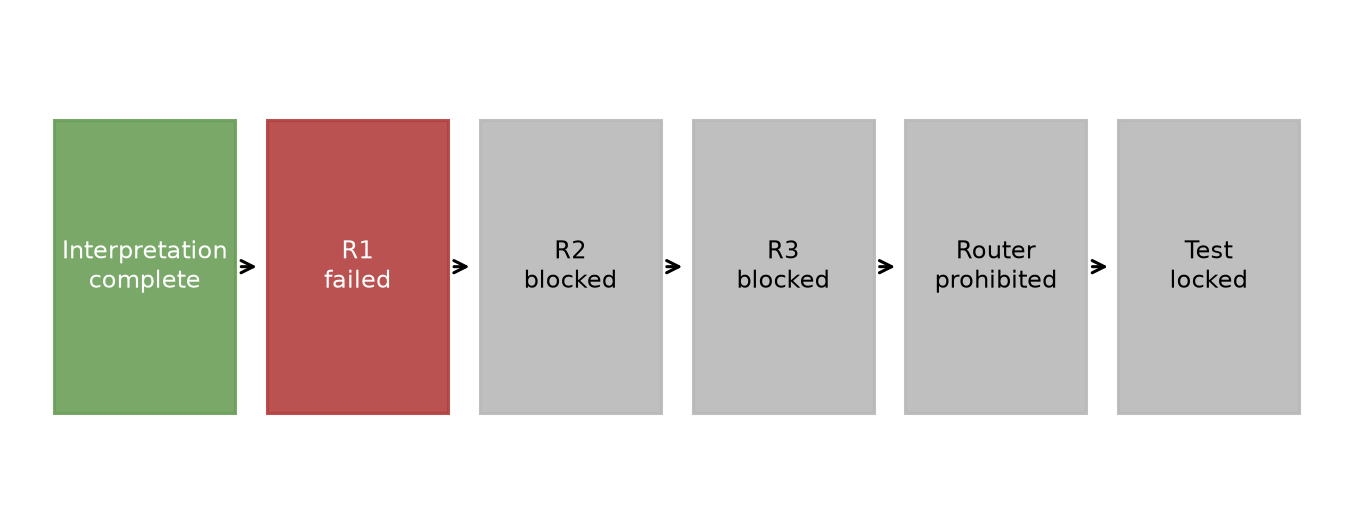
\includegraphics[width=.95\textwidth]{figures/phase3_gate_state_flow.png}
\caption{Phase 3 state flow. R1 proposal quality fails, so downstream SAM refinement, oracle analysis, router training, and formal tests are blocked by protocol.}
\label{fig:gate_flow}
\end{figure*}

\section{Results}

\subsection{Phase 2D Interpretation Audit}

The Phase 2D audit supports a narrowed interpretation. P3 grouped sparse points fail against both random-coordinate and alternative-reference controls. P4 privileged union boxes remain positive, showing that the broad SAM backbone failure claim would be too strong. Table~\ref{tab:control_decomposition} decomposes the C1/C2 controls and relabels C2 as an alternative-reference control for scientific discussion, without modifying the original historical CSVs.

\begin{table*}[t]
\centering
\small
\caption{C1/C2 decomposition over all Phase 2D prompt families. C2 is retained historically but interpreted as an alternative-reference control.}
\label{tab:control_decomposition}
\begin{tabular}{llllll}
\hline
Segmenter & Prompt & P - C1 & P - C2 & C1 - C2 & C2 label \\
\hline
SAM-B & P1 & -0.043 & -0.096 & -0.053 & alternative\_reference\_control \\
SAM-B & P2 & -0.084 & -0.043 & 0.041 & alternative\_reference\_control \\
SAM-B & P3 & -0.160 & -0.156 & 0.003 & alternative\_reference\_control \\
SAM-B & P4 & 0.044 & 0.064 & 0.020 & alternative\_reference\_control \\
SAM-B & P5 & -0.201 & -0.099 & 0.102 & alternative\_reference\_control \\
SAM-L & P1 & 0.082 & -0.058 & -0.141 & alternative\_reference\_control \\
SAM-L & P2 & 0.001 & 0.012 & 0.011 & alternative\_reference\_control \\
SAM-L & P3 & -0.074 & -0.119 & -0.045 & alternative\_reference\_control \\
SAM-L & P4 & 0.039 & 0.095 & 0.056 & alternative\_reference\_control \\
SAM-L & P5 & 0.049 & -0.016 & -0.065 & alternative\_reference\_control \\
\hline
\end{tabular}
\end{table*}


\begin{figure}[t]
\centering
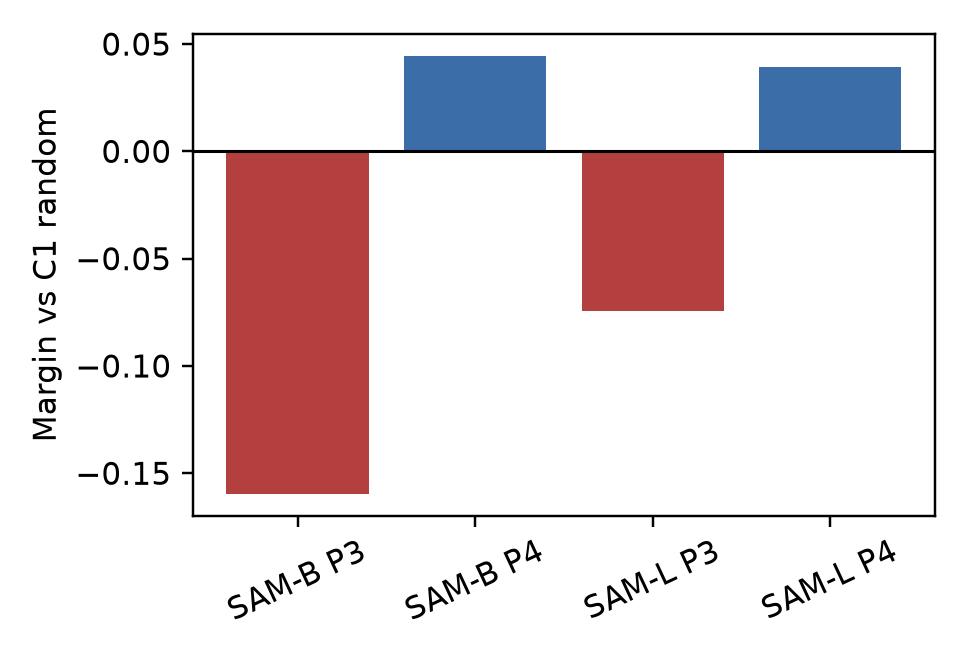
\includegraphics[width=\columnwidth]{figures/phase2d_point_vs_region_upper_bound.png}
\caption{P3 grouped points have negative margins, while privileged P4 region boxes are positive. This motivates a region-prompt pivot but does not establish an automatic method.}
\label{fig:p3_p4}
\end{figure}

\begin{figure}[t]
\centering
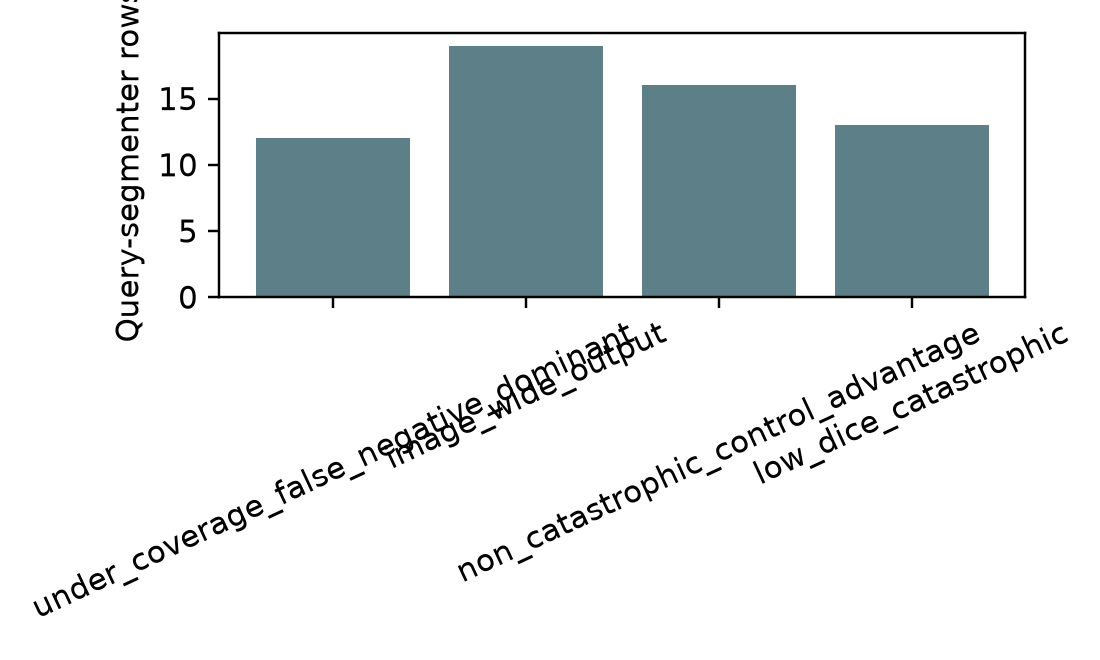
\includegraphics[width=\columnwidth]{figures/p3_failure_taxonomy.png}
\caption{P3 failure taxonomy from existing Phase 2D artifacts. Failure modes include under-coverage and image-wide outputs, consistent with a prompt-interface problem.}
\label{fig:p3_failure_taxonomy}
\end{figure}

\begin{figure*}[t]
\centering
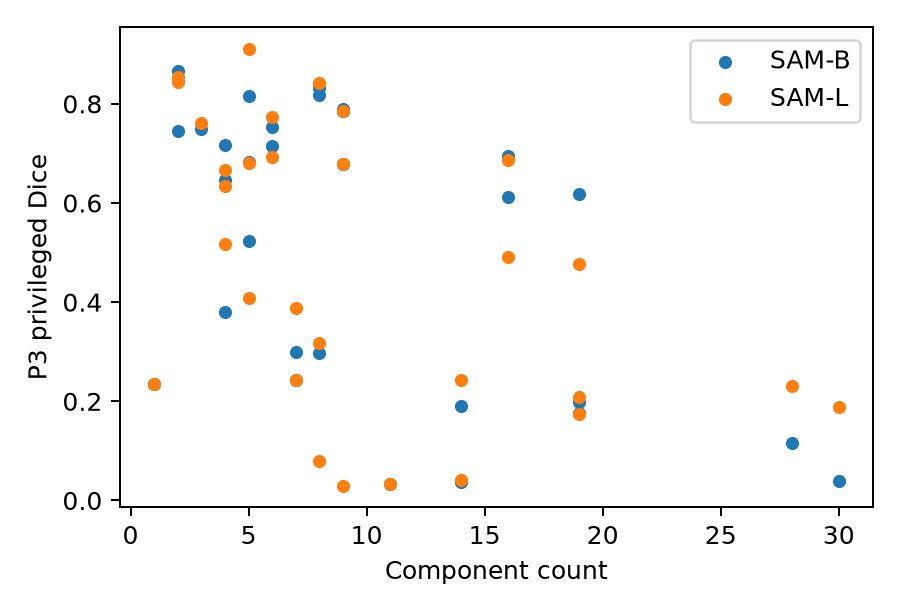
\includegraphics[width=.48\textwidth]{figures/phase2d_dice_vs_component_count.png}
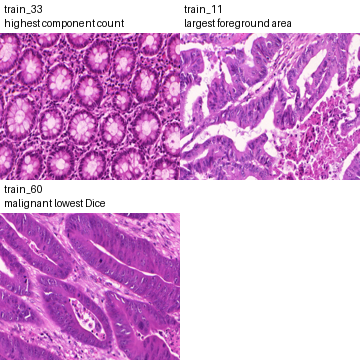
\includegraphics[width=.48\textwidth]{figures/phase2d_representative_failure_panels.png}
\caption{Existing Phase 2D failure diagnostics reused without new SAM inference. Left: grouped-point Dice varies with component structure. Right: representative failure panels selected by the Phase 2D audit rule, not by post-hoc favorable case selection.}
\label{fig:phase2d_failure_panels}
\end{figure*}

These visual diagnostics are included to prevent an overly broad backbone-failure interpretation. Some failures are under-coverage errors, where the grouped point interface captures only sparse parts of a whole-image gland mask. Other failures are image-wide outputs, where the prompt interface does not constrain SAM in a useful way. In both cases, the failure is compatible with a bad prompt representation even when the coordinate and cost audits pass.

\subsection{Gate R1 Proposal Quality}

Table~\ref{tab:r1_quality} reports the strict-validation Gate R1 results. No automatic family passes. R03 automatic union box is the strongest route by mean metric, but its improvement over size-matched random boxes is only 0.026 and its win rate is 0.200. R00 direct matching mask is precise but has low recall and low raw Dice. R04 and R05 are too small and under-cover glands.

\begin{table*}[t]
\centering
\small
\caption{Gate R1 proposal quality on 30 strict-validation queries. No automatic family passed the pre-registered thresholds.}
\label{tab:r1_quality}
\begin{tabular}{lllllllll}
\hline
Family & Route & Metric & Control & Improvement & Win & Recall & Empty & Status \\
\hline
R00 direct matching mask & mask & 0.179 & 0.595 & -0.416 & 0.067 & 0.100 & 0.000 & FAIL \\
R03 automatic union box & box & 0.745 & 0.719 & 0.026 & 0.200 & 0.791 & 0.000 & FAIL \\
R04 automatic largest component box & box & 0.019 & 0.017 & 0.002 & 0.100 & 0.030 & 0.000 & FAIL \\
R05 automatic top3 component boxes & box & 0.272 & 0.255 & 0.017 & 0.167 & 0.063 & 0.000 & FAIL \\
\hline
\end{tabular}
\end{table*}


\begin{figure*}[t]
\centering
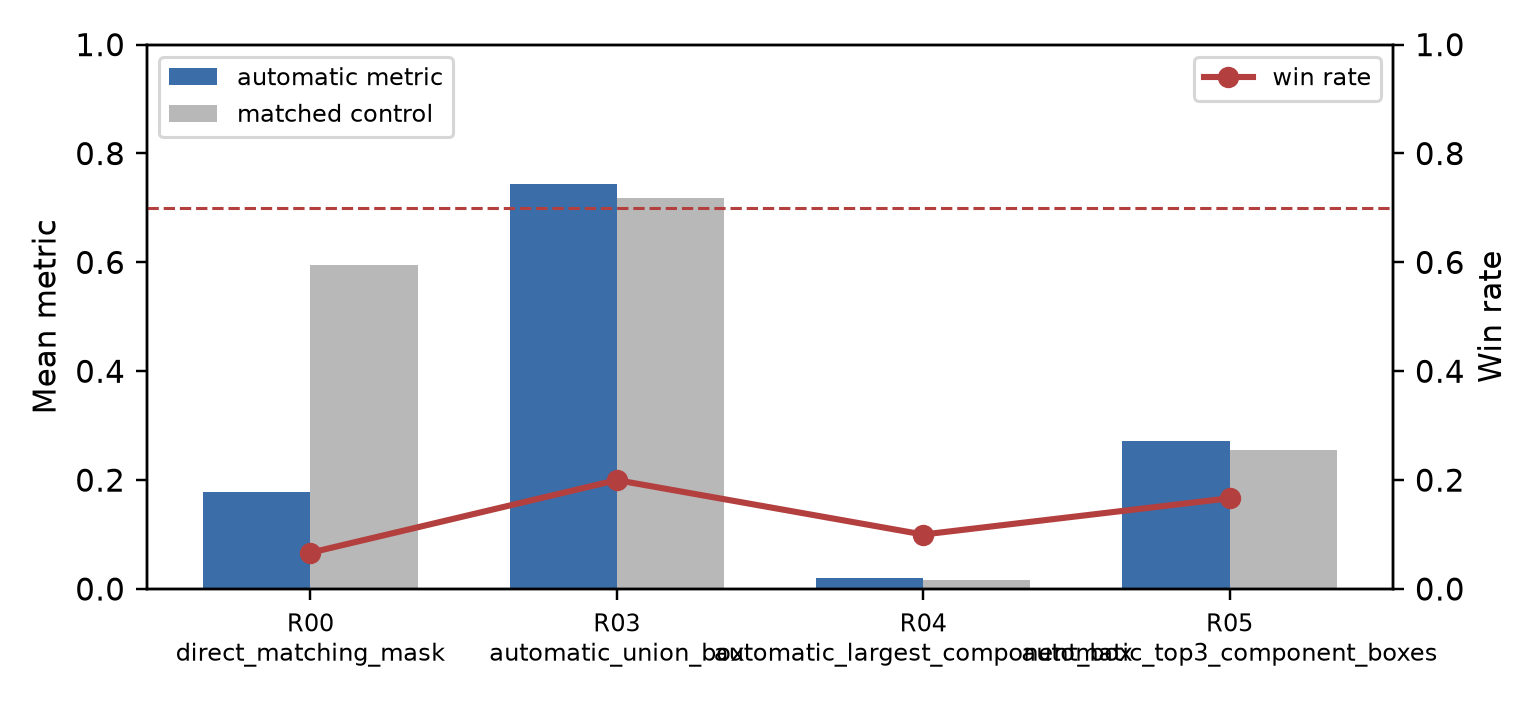
\includegraphics[width=.48\textwidth]{figures/r1_family_metrics.png}
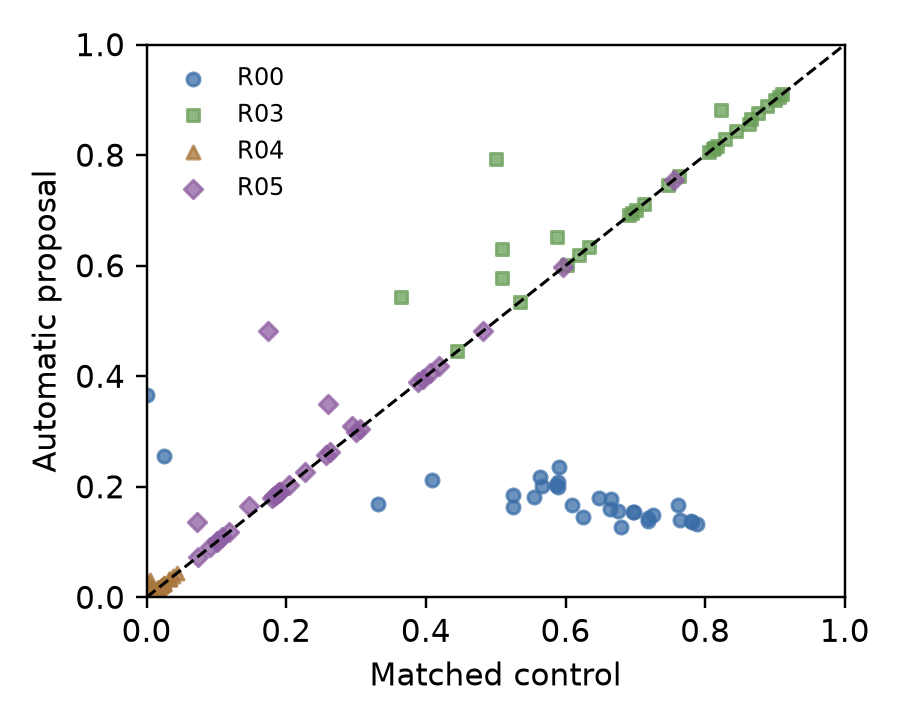
\includegraphics[width=.48\textwidth]{figures/r1_automatic_vs_control_scatter.png}
\caption{Gate R1 diagnostics. Left: automatic proposal metrics and matched controls by family, with the 0.70 win-rate threshold shown. Right: query-level automatic-versus-control scatter; most points do not clear the diagonal by a meaningful margin.}
\label{fig:r1_diagnostics}
\end{figure*}

\begin{figure}[t]
\centering
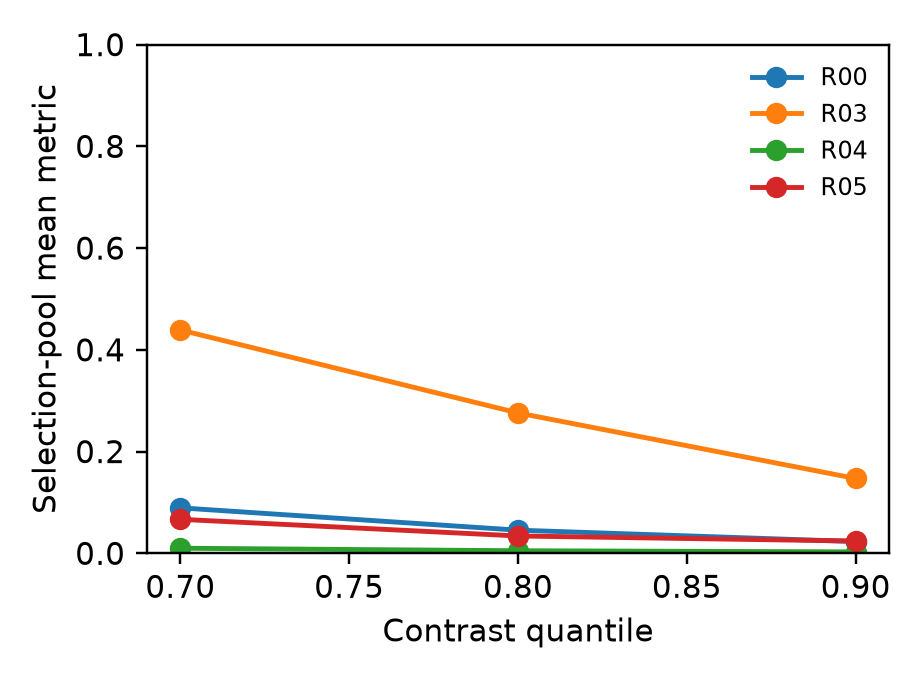
\includegraphics[width=\columnwidth]{figures/r1_parameter_grid_curves.png}
\caption{Internal selection-pool parameter grid summary. The selected configurations use the fixed pre-registered grid; strict validation is not used to choose parameters.}
\label{fig:r1_grid}
\end{figure}

\subsection{Blocked Downstream Quantities}

Because R1 fails before new SAM region inference, SAM-refined Dice, SAM gain, upper-bound recovery, R3 oracle gap, router comparison, and formal test results are not measured. Table~\ref{tab:downstream_status} records these as blocked quantities, not missing favorable results.

\begin{table*}[t]
\centering
\small
\caption{Downstream Phase 3 quantities are explicitly blocked by R1 failure rather than silently omitted.}
\label{tab:downstream_status}
\begin{tabular}{lll}
\hline
Stage & State & Reported value \\
\hline
R2 SAM region viability & BLOCKED\_BY\_R1\_FAILURE & not run \\
SAM gain & BLOCKED\_BY\_R1\_FAILURE & N/A \\
Region recovery & BLOCKED\_BY\_R1\_FAILURE & N/A \\
R3 oracle gap & BLOCKED\_BY\_R1\_FAILURE & N/A \\
Router & PROHIBITED\_BY\_R1\_FAILURE & not trained \\
Formal test & PROHIBITED\_BY\_R1\_FAILURE & testA/testB locked \\
\hline
\end{tabular}
\end{table*}

\begin{table*}[t]
\centering
\small
\caption{Compute, access, and final-state ledger for Phase 3.}
\label{tab:compute_access}
\begin{tabular}{ll}
\hline
Item & Value \\
\hline
Phase 3 GPU hours & 0.029398 \\
Budget & 40 \\
testA & LOCKED\_UNUSED \\
testB & LOCKED\_UNUSED \\
Preregistration commit & 471f529 \\
Final state & STOP\_GLAS\_REGION\_PROPOSAL\_FAILURE \\
\hline
\end{tabular}
\end{table*}


\section{Discussion}

The strongest evidence in Phase 3 is negative but useful. It shows that a reference-conditioned region-prompt route cannot be assumed simply because privileged GT boxes work. The frozen DINOv2-L/local-peaks evidence can find high-precision fragments, yet the fragments do not produce region proposals that beat matched random controls with sufficient query-level consistency. The gap between privileged P4 and automatic R1 therefore becomes an automatic-proposal gap, not a SAM refinement result.

This distinction protects the scientific claim. If we had skipped R1 and run SAM on weak proposals, a later Dice failure would conflate proposal quality with the segmenter's ability to refine a region. Conversely, if a few qualitative examples looked good, they would not justify method claims under the pre-registered win-rate and matched-control thresholds. R1 forces the pipeline to prove that the automatic prompt input is already meaningful before spending SAM calls.

The result also reframes AdaPromptSet. The original budget-constrained prompt-set selection story remains too strong for the available evidence. A more accurate direction is reference-conditioned prompt representation analysis: determining when a point, box, mask, direct matching mask, or deterministic region is justified by frozen evidence. In this GlaS setting, the answer is that the tested automatic region proposals are insufficient.

One practical consequence is that the next legal experiment cannot be a quiet threshold expansion or per-query strict-validation tweak. It would require a new pre-registered rescue protocol using only allowed development data or a new external data source, with explicit data-manifest and method gates. Without that, the correct final state is \texttt{STOP\_GLAS\_REGION\_PROPOSAL\_FAILURE}.

\section{Limitations}

This report is intentionally narrower than a success-method paper. It does not evaluate SAM-B automatic region prompts because R1 fails before SAM inference. It does not evaluate SAM-L replication, R3 oracle gap, a learned router, or formal testA/testB performance. Those omissions are protocol consequences, not hidden negative results.

The R1 implementation uses sparse candidate evidence from the frozen local-peaks redesign rather than cached full dense maps for every reference. The report therefore supports a statement about the tested frozen local-peaks-derived proposals, not all possible dense matching-map segmentations. The region bank is finite and pre-registered; it does not cover learned proposal models, trainable medical segmenters, SAM-H, SAM2, MedSAM, or unrestricted search.

The GT upper-bound rows are privileged and cannot be mixed with automatic results. They remain useful for interpreting the prompt interface, but they do not prove deployable automatic region prompting. Finally, the 30 strict-validation queries are a validation gate, not a formal test. testA/testB remain locked and unused.

\section{Reproducibility and Audit Trail}

\subsection{Commit and Artifact Boundaries}

Phase 3 starts from the Phase 2D artifact commit \texttt{93b319e}. The pre-registration commit is \texttt{471f529}, created before the internal candidate calibration and before Gate R1 evaluation. This matters because the R1 threshold grid, action bank, data roles, claim registry, and access rules were already fixed when strict validation was evaluated. The final state is therefore not a retrospective interpretation of a failed experiment; it is the direct output of the pre-registered state machine.

The required Phase 3 documents are present as versioned project artifacts: the goal read receipt, scientific pivot, Gate-D interpretation addendum, region prompt protocol, exposure audit, claim registry, gate status, compute ledger, protocol snapshot, and input hashes. The split artifacts freeze the 40 calibration images, 15 internal selection images, and reference episodes. The R1 artifacts include full parameter-grid results, selected global configurations, query-level metrics, family summaries, and a JSON/Markdown gate summary.

\subsection{Why R2 Was Not Run}

The most important reproducibility decision is the absence of R2. R2 would have measured SAM-B automatic region prompt viability, SAM gain, and recovery relative to privileged GT upper bounds. Running it after R1 failure would violate the protocol because the automatic prompt input did not first clear proposal-quality thresholds. This is not an efficiency shortcut. It prevents a weak automatic proposal from being laundered into a segmenter claim, and it prevents qualitative cherry-picking after observing strict-validation behavior.

The same logic applies downstream. R3 needs R2-passing automatic actions to construct a legal region-action utility matrix. The router needs R3 to demonstrate that query-level prompt representation preferences exist and are predictable. Formal testA/testB access needs either a validated router, a frozen deterministic region method, or a frozen direct-mask method. None of those states was reached, so all downstream quantities are recorded as blocked.

\subsection{Claim Mapping}

The allowed claim is limited to the gate evidence: frozen matching evidence and sparse local-peak candidates did not produce region proposals that beat pre-registered R1 controls on GlaS strict validation; the automatic region prompt route stops before SAM refinement. The forbidden claims are correspondingly explicit. The paper does not claim that automatic region prompting works, that SAM refinement adds value, that a region oracle gap exists, that a router improves performance, or that formal test performance has been measured.

This mapping is conservative but useful. It converts an experimental failure into a boundary condition for prompt-interface research. The data show that the region interface is viable under privileged GT boxes, but the tested automatic proposal generator cannot supply that interface reliably enough. Any future positive result must therefore solve the automatic proposal gap under a new pre-registered protocol rather than tune the current strict-validation failure.

\subsection{Command-Level Reproduction}

The reproducible Phase 3 path is the following script sequence, each invoked with the project root fixed to \texttt{D:/SAM/adapromptset}: interpretation audit, 40/15 split builder, candidate-pilot evidence export, Gate R1 runner, and Phase 3 paper asset export.

The first two commands are CPU-only artifact and manifest steps. The candidate-pilot command writes frozen matching evidence for the internal protocol and is logged as a Gate-C-style artifact producer, not as the R1 decision. The R1 command writes the unique Phase 3 stopping state. The paper asset exporter reads only those artifacts and emits the tables and figures used in this PDF.

\section{Conclusion}

Phase 3 preserves the historical Phase 2D operational failure while correcting the scientific interpretation. Grouped sparse point prompting failed; privileged region prompts show that the region interface remains viable in principle. The automatic region route, however, fails at Gate R1: frozen matching evidence and local-peaks proposals do not produce region proposals that clear matched-control thresholds on GlaS strict validation. The final state is \texttt{STOP\_GLAS\_REGION\_PROPOSAL\_FAILURE}. No automatic region prompting success, SAM refinement gain, oracle gap, router improvement, or formal test result is claimed.

The useful outcome is therefore a boundary, not a benchmark win. Under the tested frozen matcher, fixed local-peaks evidence, and pre-registered proposal bank, the prompt representation bottleneck appears before SAM refinement. Future work must first demonstrate a legal automatic proposal improvement under a new frozen protocol before revisiting region-prompt viability or prompt-type routing.

\section*{Artifact Index}

The authoritative Phase 3 final report is stored in the Phase 3 final-report Markdown and JSON files. Gate R1 evidence is stored in the Phase 3 GlaS R1 report directory. The interpretation audit is stored in the Phase 3 interpretation-audit report directory. The fixed 40/15 internal split is stored in the Phase 3 manifests. The region bank is stored as the GlaS region-bank v1 JSON/YAML pair. This PDF and its source are stored under the Phase 3 paper directory. The final test access state is unchanged: GlaS testA and testB are locked and unused.


\begin{thebibliography}{9}
\bibitem{sam}
Kirillov et al. Segment Anything. ICCV, 2023.

\bibitem{dinov2}
Oquab et al. DINOv2: Learning Robust Visual Features without Supervision. TMLR, 2024.

\bibitem{glas}
Sirinukunwattana et al. Gland Segmentation in Colon Histology Images: The GlaS Challenge Contest. Medical Image Analysis, 2017.

\bibitem{medsam}
Ma et al. Segment Anything in Medical Images. Nature Communications, 2024.

\bibitem{matcher}
Liu et al. One-shot object localization and reference-guided segmentation with frozen visual features. Reference-guided segmentation family, 2023.
\end{thebibliography}

\end{document}
